% ========================================
%	Header einbinden
% ========================================

\documentclass[bibtotoc,titlepage]{scrartcl}

% Deutsche Spracheinstellungen
\usepackage[ngerman,german]{babel, varioref}
\usepackage[T1]{fontenc}
\usepackage[utf8]{inputenc}

%\usepackage{marvosym}

\usepackage{amsfonts}
\usepackage{amssymb}
\usepackage{amsmath}
\usepackage{amscd}
\usepackage{amstext}
\usepackage{float}
\usepackage{caption}
\usepackage{wrapfig}
\usepackage{setspace}
\usepackage{threeparttable}
\usepackage{footnote}

\newfloat{formel}{htbp}{for}
\floatname{formel}{Formel}


\usepackage{longtable}

%\usepackage{bibgerm}

\usepackage{footnpag}

\usepackage{ifthen}                 %%% package for conditionals in TeX
\usepackage[amssymb]{SIunits}
%Fr textumflossene Bilder und Tablellen
%\usepackage{floatflt} - veraltet

%Fr Testzwecke aktivieren, zeigt labels und refs im Text an.
%\usepackage{showkeys}

% Abstand zwischen zwei Abs�zen nach DIN (1,5 Zeilen)
% \setlength{\parskip}{1.5ex plus0.5ex minus0.5ex}

% Einrckung am Anfang eines neuen Absatzes nach DIN (keine)
%\setlength{\parindent}{0pt}

% R�der definieren
% \setlength{\oddsidemargin}{0.3cm}
% \setlength{\textwidth}{15.6cm}

% bessere Bildunterschriften
%\usepackage[center]{caption2}


% Probleml�ungen beim Umgang mit Gleitumgebungen
\usepackage{float}

% Nummeriert bis zur Strukturstufe 3 (also <section>, <subsection> und <subsubsection>)
%\setcounter{secnumdepth}{3}

% Fhrt das Inhaltsverzeichnis bis zur Strukturstufe 3
%\setcounter{tocdepth}{3}

\usepackage{exscale}

\newenvironment{dsm} {\begin{displaymath}} {\end{displaymath}}
\newenvironment{vars} {\begin{center}\scriptsize} {\normalsize \end{center}}


\newcommand {\en} {\varepsilon_0}               % Epsilon-Null aus der Elektrodynamik
\newcommand {\lap} {\; \mathbf{\Delta}}         % Laplace-Operator
\newcommand {\R} { \mathbb{R} }                 % Menge der reellen Zahlen
\newcommand {\e} { \ \mathbf{e} }               % Eulersche Zahl
\renewcommand {\i} { \mathbf{i} }               % komplexe Zahl i
\newcommand {\N} { \mathbb{N} }                 % Menge der nat. Zahlen
\newcommand {\C} { \mathbb{C} }                 % Menge der kompl. Zahlen
\newcommand {\Z} { \mathbb{Z} }                 % Menge der kompl. Zahlen
\newcommand {\limi}[1]{\lim_{#1 \rightarrow \infty}} % Limes unendlich
\newcommand {\sumi}[1]{\sum_{#1=0}^\infty}
\newcommand {\rot} {\; \mathrm{rot} \,}         % Rotation
\newcommand {\grad} {\; \mathrm{grad} \,}       % Gradient
\newcommand {\dive} {\; \mathrm{div} \,}        % Divergenz
\newcommand {\dx} {\; \mathrm{d} }              % Differential d
\newcommand {\cotanh} {\; \mathrm{cotanh} \,}   %Cotangenshyperbolicus
\newcommand {\asinh} {\; \mathrm{areasinh} \,}  %Area-Sinus-Hyp.
\newcommand {\acosh} {\; \mathrm{areacosh} \,}  %Area-Cosinus-H.
\newcommand {\atanh} {\; \mathrm{areatanh} \,}  %Area Tangens-H.
\newcommand {\acoth} {\; \mathrm{areacoth} \,}  % Area-cotangens
\newcommand {\Sp} {\; \mathrm{Sp} \,}
\newcommand {\mbe} {\stackrel{\text{!}}{=}}     %Must Be Equal
\newcommand{\qed} { \hfill $\square$\\}
\renewcommand{\i} {\imath}
\def\captionsngerman{\def\figurename{\textbf{Abb.}}}

%%%%%%%%%%%%%%%%%%%%%%%%%%%%%%%%%%%%%%%%%%%%%%%%%%%%%%%%%%%%%%%%%%%%%%%%%%%%
% SWITCH FOR PDFLATEX or LATEX
%%%%%%%%%%%%%%%%%%%%%%%%%%%%%%%%%%%%%%%%%%%%%%%%%%%%%%%%%%%%%%%%%%%%%%%%%%%%
%%%
\ifx\pdfoutput\undefined %%%%%%%%%%%%%%%%%%%%%%%%%%%%%%%%%%%%%%%%% LATEX %%%
%%%
\usepackage[dvips]{graphicx}       %%% graphics for dvips
\DeclareGraphicsExtensions{.eps,.ps}   %%% standard extension for included graphics
\usepackage[ps2pdf]{thumbpdf}      %%% thumbnails for ps2pdf
\usepackage[ps2pdf,                %%% hyper-references for ps2pdf
bookmarks=true,%                   %%% generate bookmarks ...
bookmarksnumbered=true,%           %%% ... with numbers
hypertexnames=false,%              %%% needed for correct links to figures !!!
breaklinks=true,%                  %%% breaks lines, but links are very small
linkbordercolor={0 0 1},%          %%% blue frames around links
pdfborder={0 0 112.0}]{hyperref}%  %%% border-width of frames
%                                      will be multiplied with 0.009 by ps2pdf
%
\hypersetup{ pdfauthor   = {Hannes Franke; Julius Tilly},
pdftitle    = {V301 Innenwiderstand und Leistungsanpassung}, pdfsubject  = {Protokoll FP}, pdfkeywords = {V301, Innenwiderstand, Leistungsanpassung},
pdfcreator  = {LaTeX with hyperref package}, pdfproducer = {dvips
+ ps2pdf} }
%%%
\else %%%%%%%%%%%%%%%%%%%%%%%%%%%%%%%%%%%%%%%%%%%%%%%%%%%%%%%%%% PDFLATEX %%%
%%%
\usepackage[pdftex]{graphicx}      %%% graphics for pdfLaTeX
\DeclareGraphicsExtensions{.pdf}   %%% standard extension for included graphics
\usepackage[pdftex]{thumbpdf}      %%% thumbnails for pdflatex
\usepackage[pdftex,                %%% hyper-references for pdflatex
bookmarks=true,%                   %%% generate bookmarks ...
bookmarksnumbered=true,%           %%% ... with numbers
hypertexnames=false,%              %%% needed for correct links to figures !!!
breaklinks=true,%                  %%% break links if exceeding a single line
linkbordercolor={0 0 1},
linktocpage]{hyperref} %%% blue frames around links
%                                  %%% pdfborder={0 0 1} is the default
\hypersetup{
pdftitle    = {V301 Innenwiderstand und Leistungsanpassung}, 
pdfsubject  = {Protokoll AP}, 
pdfkeywords = {V301, Innenwiderstand, Leistungsanpassung},
pdfsubject  = {Protokoll AP},
pdfkeywords = {V301, Innenwiderstand, Leistungsanpassung}}
%                                  %%% pdfcreator, pdfproducer,
%                                      and CreationDate are automatically set
%                                      by pdflatex !!!
\pdfadjustspacing=1                %%% force LaTeX-like character spacing
\usepackage{epstopdf}
%
\fi %%%%%%%%%%%%%%%%%%%%%%%%%%%%%%%%%%%%%%%%%%%%%%%%%%% END OF CONDITION %%%
%%%%%%%%%%%%%%%%%%%%%%%%%%%%%%%%%%%%%%%%%%%%%%%%%%%%%%%%%%%%%%%%%%%%%%%%%%%%
% seitliche Tabellen und Abbildungen
%\usepackage{rotating}
\usepackage{ae}
\usepackage{
  array,
  booktabs,
  dcolumn
}
\makeatletter 
  \renewenvironment{figure}[1][] {% 
    \ifthenelse{\equal{#1}{}}{% 
      \@float{figure} 
    }{% 
      \@float{figure}[#1]% 
    }% 
    \centering 
  }{% 
    \end@float 
  } 
  \makeatother 


  \makeatletter 
  \renewenvironment{table}[1][] {% 
    \ifthenelse{\equal{#1}{}}{% 
      \@float{table} 
    }{% 
      \@float{table}[#1]% 
    }% 
    \centering 
  }{% 
    \end@float 
  } 
  \makeatother 
%\usepackage{listings}
%\lstloadlanguages{[Visual]Basic}
%\allowdisplaybreaks[1]
%\usepackage{hycap}
%\usepackage{fancyunits}
\usepackage{multirow}
\usepackage{color}

% ========================================
%	Angaben für das Titelblatt
% ========================================

\title{Versuch 28 - Elektronenspinresonanz\\% Titel des Versuchs 
\large TU Dortmund, Fakultät Physik\\ 
\normalsize Fortgeschrittenen-Praktikum}

\author{Jan Adam\\			% Name Praktikumspartner A
{\small \href{jan.adam@tu-dortmund.de}{jan.adam@tu-dortmund.de}}	% Erzeugt interaktiven einen Link
\and						% um einen weiteren Author hinzuzfügen
Dimitrios Skodras\\					% Name Praktikumspartner B
{\small \href{dimitrios.skodras@tu-dortmund.de}{dimitrios.skodras@tu-dortmund.de}}		% Erzeugt interaktiven einen Link
}
\date{30. April 2014}				% Das Datum der Versuchsdurchführung

% ========================================
%	Das Dokument beginnt
% ========================================

\begin{document}

% ========================================
%	Titelblatt erzeugen
% ========================================

\maketitle					% Jetzt wird die Titelseite erzeugt
\thispagestyle{empty} 				% Weder Kopfzeile noch Fußzeile

% ========================================
%	Der Vorspann
% ========================================

%\newpage					% Wenn Verzeichnisse auf einer neuen Seite beginnen sollen
%\pagestyle{empty}				% Weder Kopf- noch Fußzeile für Verzeichnisse

\tableofcontents

%\newpage					% eine neue Seite
%\thispagestyle{empty}				% Weder Kopf- noch Fußzeile für Verzeichnisse
%\listoffigures					% Abbildungsverzeichnis

%\newpage					% eine neue Seite
%\thispagestyle{empty}				% Weder Kopf- noch Fußzeile für Verzeichnisse
%\listoftables					% Tabellenverzeichnis
\newpage					% eine neue Seite


% ========================================
%	Kapitel
% ========================================

%\section{Einleitung}				% Bei Bedarf

\section{Theorie}
\setcounter{page}{1}

\section{Durchführung}

\section{Auswertung}
\subsection{Kalibrierung der Messachsen}
\label{sec_Kalib}
Zur Bestimmung der für die Auswertung relevanten Resonanzstellen, ist es erforderlich, die im Anhang aufgeführten Messkurven entlang der X-Achse
nach den gemessenen Spannungen $U_\text{Rampe}$ = $U_\text{R}$ zu kalibrieren. 
\begin{equation}
 U_\text{R} = m\cdot x + U_0
\end{equation}

Hierzu dienen die Werte aus den Tabellen \ref{tab_xAxisKalib15MHz} bis
\ref{tab_xAxisKalib30MHz}. Rot geschriebene Zahlen zeichnen hier die Resonanzstelle
\renewcommand{\arraystretch}{1.2}
\begin{table}[H]
 \begin{tabular}{c|c|c|c||c|c|c|c}
  $x$ in cm & $y$ in cm & $U_\text{R}$ in V & $U_\text{B} $ in mV & $x$ in cm & $y$ in cm & $U_\text{R}$ in V & $U_\text{B}$ in mV \\
 \hline
 0,0&	0,0&	10,0&	181,0&	0,0&	0,0&		5,0&	173,0\\
4,0&	0,0&	14,1&	181,0&	4,0&	0,0&		9,8&	173,0\\
7,0&	0,3&	17,2&	183,5&	7,0&	0,2&		13,5&	174,0\\
8,0&	0,5&	18,2&	185,2&	9,0&	0,5&		15,9&	175,5\\
9,0&	0,6&	\textcolor{red}{19,2}&	\textcolor{red}{186,0}&	10,0&	0,6&		\textcolor{red}{17,1}&	\textcolor{red}{176,0}\\
10,0&	0,6&	\textcolor{red}{20,2}&	\textcolor{red}{186,0}&	11,0&	0,5&		18,3&	175,5\\
11,0&	0,5&	21,3&	185,2&	12,0&	0,4&		19,5&	175,0\\
12,0&	0,4&	22,3&	184,3&	13,0&	0,2&		20,8&	174,0\\
14,0&	0,1&	24,3&	181,8&	16,0&	0,0&		24,4&	173,0\\
17,0&	0,0&	27,4&	181,0&	19,8&	0,0&		29,0&	173,0\\ 
21,5&	-0,1&	32,0&	180,2&	&	&		&	\\

 \end{tabular}
 \caption{Messkurven bei $\nu_e$ = 14,798 kHz; links $B_\text{parallel}$ und rechts $B_\text{parallel}$}
 \label{tab_xAxisKalib15MHz}
\end{table}
\begin{table}[H]
 \begin{tabular}{c|c|c|c||c|c|c|c}
  $x$ in cm & $y$ in cm & $U_\text{R}$ in V & $U_\text{B} $ in mV & $x$ in cm & $y$ in cm & $U_\text{R}$ in V & $U_\text{B}$ in mV \\
 \hline
0,0	&0,0&	15,0&	182,8	&0,0&	0&	14,0&	156,0\\
2,0&	0,2&	16,8&	183,9&	3,0&	0&	17,5&	156,0\\
4,0&	0,3&	18,7&	184,5&	6,0&	0,3&	20,9&	158,1\\
6,0&	0,9&	20,5&	187,8&	7,0&	0,5&	22,1&	159,6\\
8,0&	2,3&	22,4&	195,5&	8,0&	0,7&	\textcolor{red}{23,2}&	\textcolor{red}{161,0}\\
9,0&	3,1&	23,3&	199,9&	9,0&	0,6&	24,4&	160,3\\
10,0&	3,9&	24,2&	204,4&	10,0&	0,6&	25,5&	160,3\\
10,5&	4,6&	24,7&	208,2&	12,0&	0,2&	27,8&	157,4\\
11,0&	4,9&	25,1&	209,9&	16,5&	0,1&	33,0&	156,7\\
11,5&	5,1&	\textcolor{red}{25,6}&	\textcolor{red}{211,0}&		&&		&\\
12,0&	5,1&	\textcolor{red}{26,1}&	\textcolor{red}{211,0}&		&&		&\\
12,5&	4,9&	26,5&	209,9&		&&		&\\
13,0&	4,6&	27,0&	208,2&		&&		&\\
13,5&	4,3&	27,4&	206,6&		&&		&\\
14,0&	3,9&	27,9&	204,4&		&&		&\\
15,0&	3,0&	28,8&	199,4&		&&		&\\
16,0&	2,6&	29,7&	197,2&		&&		&\\
17,0&	2,1&	30,7&	194,4&		&&		&\\
19,0&	1,4&	32,5&	190,6&		&&		& \\

 \end{tabular}
 \caption{Messkurven bei $\nu_e$ = 19,448 kHz; links $B_\text{parallel}$ und rechts $B_\text{parallel}$}
 \label{tab_xAxisKalib20MHz}
\end{table}
\begin{table}[H]
 \begin{tabular}{c|c|c|c||c|c|c|c}
  $x$ in cm & $y$ in cm & $U_\text{R}$ in V & $U_\text{B} $ in mV & $x$ in cm & $y$ in cm & $U_\text{R}$ in V & $U_\text{B}$ in mV \\
 \hline
0,0 &	0,0&	23,0&	177,0&	0,0&	0,7&	17,0&	211,0\\
2,0&	0,1&	25,1&	177,8&	1,0&	0,0&	18,3&	205,0\\
4,0&	0,7&	27,1&	182,4&	2,0&	0,0&	19,6&	205,0\\
5,0&	0,9&	28,1&	184,0&	3,0&	0,3&	20,9&	207,6\\
6,0&	1,4&	29,2&	187,9&	4,0&	0,9&	22,2&	212,7\\
6,5&	1,6&	29,7&	189,4&	5,0&	1,6&	23,5&	218,7\\
7,0&	1,7&	30,2&	190,2&	6,0&	2,8&	24,9&	229,0\\
7,5&	1,8&	\textcolor{red}{30,7}&	\textcolor{red}{191,0}&	7,0&	4,5&	26,2&	243,6\\
8,0&	1,8&	\textcolor{red}{31,2}&	\textcolor{red}{191,0}&	7,5&	5,4&	26,8&	251,3\\
9,0&	1,4&	32,3&	187,9&	8,0&	6,3&	27,5&	259,0\\
10,0&	1,0&	33,3&	184,8&	8,5&	6,9&	28,1&	264,1\\
11,0&	0,8&	34,3&	183,2&	9,0&	7,0&	\textcolor{red}{28,8}&	\textcolor{red}{265,0}\\
13,0&	0,3&	36,4&	179,3&	9,5&	6,9&	29,4&	264,1\\
15,0&	0,1&	38,4&	177,8&	10,0&	6,5&	30,1&	260,7\\
17,5&	-0,1&	41,0&	176,2&	10,5&	5,6&	30,8&	253,0\\
&	&	&	&	11,0&	4,6&	31,4&	244,4\\
&	&	&	&	11,5&	3,8&	32,1&	237,6\\
&	&	&	&	13,0&	2,5&	34,0&	226,4\\
&	&	&	&	14,0&	1,4&	35,3&	217,0\\
&	&	&	&	14,5&	1,1&	36,0&	214,4\\
&	&	&	&	16,8&	1,1&	39,0&	214,4 \\

 \end{tabular}
 \caption{Messkurven bei $\nu_e$ = 23,888 kHz; links $B_\text{parallel}$ und rechts $B_\text{parallel}$}
 \label{tab_xAxisKalib24MHz}
\end{table}
\begin{table}[H]
 \begin{tabular}{c|c|c|c||c|c|c|c}
  $x$ in cm & $y$ in cm & $U_\text{R}$ in V & $U_\text{B} $ in mV & $x$ in cm & $y$ in cm & $U_\text{R}$ in V & $U_\text{B}$ in mV \\
 \hline
0,0 &	0,0&	24,0&	222,0&	0,0&	0,1&	26,0&	181,7\\
2,0&	0,1&	26,1&	222,7&	1,0&	0,0&	27,1&	181,0\\
4,0&	0,2&	28,3&	223,4&	1,5&	0,1&	27,6&	181,7\\
6,0&	0,5&	30,4&	225,4&	2,0&	0,3&	28,2&	183,1\\
7,0&	0,7&	31,5&	226,8&	4,0&	0,6&	30,3&	185,1\\
8,0&	1,1&	32,6&	229,5&	5,0&	0,5&	31,4&	184,4\\
8,5&	1,5&	33,1&	232,2&	6,0&	0,8&	32,5&	186,5\\
9,0&	2,2&	33,6&	237,0&	7,0&	1,2&	33,5&	189,3\\
10,0&	2,8&	34,7&	241,1&	8,0&	1,5&	34,6&	191,3\\
10,5&	3,3&	35,3&	244,5&	8,5&	1,6&	\textcolor{red}{35,2}&	\textcolor{red}{192,0}\\
11,0&	3,6&	35,8&	246,6&	9,0&	1,6&	\textcolor{red}{35,7}&	\textcolor{red}{192,0}\\
12,0&	4,0&	36,9&	249,3&	9,5&	1,5&	36,2&	191,3\\
12,5&	4,1&	\textcolor{red}{37,4}&	\textcolor{red}{250,0}&	11,5&	0,8&	38,4&	186,5\\
13,0&	4,0&	37,9&	249,3&	12,5&	0,8&	39,5&	186,5\\
14,0&	3,5&	39,0&	245,9&	15,0&	0,4&	42,2&	183,8\\
15,0&	2,8&	40,1&	241,1&	17,0&	0,3&	44,3&	183,1\\
15,5&	2,1&	40,6&	236,3&	19,5&	0,2&	47,0&	182,4\\
16,0&	1,7&	41,1&	233,6&	&	&	&	\\
17,0&	1,3&	42,2&	230,9&	&	&	&	\\
19,0&	0,7&	44,4&	226,8&	&	&	&	\\
19,6&	0,6&	45,0&	226,1&	&	&	&	\\

 \end{tabular}
 \caption{Messkurven bei $\nu_e$ = 29,448 kHz; links $B_\text{parallel}$ und rechts $B_\text{parallel}$}
 \label{tab_xAxisKalib30MHz}
\end{table}
Hieraus ergeben sich nun die jeweiligen Kalibrierungsfaktoren in Tabelle \ref{tab_xAxisKalibTOTAL}. Mit einem Widerstand von 50 $\Omega$ lassen sich
die Rampengeneratorspannungen in Ströme $I$ umrechnen.
\begin{table}[H]
 \begin{tabular}{c|c|c|c}
  $\nu_e$ in MHz & $m$ in V/cm & $U_\text{res}$ in V & $I_\text{res}$ in mA\\
  \hline
  14,798 & 1,02 & 19,72 & 394,4 \\
  & 1,21&17,12 & 342,4\\
  19,448&0,92 &25,82 & 516,4\\
  &1,15&23,21& 464,2\\
  23,888&1,03&30,97& 619,4\\
  &1,31&28,79&575,7\\
  29,448&1,07&37,39&747,8\\
  &1,08&35,42&708,5\\
 \end{tabular}
\caption{Zusammengefasste Werte}
\label{tab_xAxisKalibTOTAL}
\end{table}

\subsection{Magnetische Flussdichte der Erde}
Mit den Ergebnissen aus Abschnitt \ref{sec_Kalib} lässt sich nun das Erdmagnetfeld bestimmen. Hierzu werden die Ströme $I_\text{res}$ aus Tabelle
\ref{tab_xAxisKalibTOTAL} nach der Gleichung für die Helmholtzspulen \eqref{eq_helmholtz.113} in magnetische Flussdichten umgerechnet, wobei der Radius
$r$ = 0,1 m und die Windungszahl N = 156 ist. Da für gleiche Frequenzen $\nu_e$ die Resonanzstellen verschieden sind, bewirkt das Erdmagnetfeld einen
Einfluss in die jeweilige Richtung, je nachdem, ob die Spule parallel oder antiparallel dazu ausgerichtet ist. Diesen Einfluss kann man ermitteln,
indem die zueinander gehörenden Flussdichten voneinander abgezogen und das Ergebnis halbiert wird
\begin{equation}
 B_\text{Erde} = \frac12 ( B_\text{par} - B_\text{antipar}).
\end{equation}
In Tabelle \ref{tab_erdMagnetfeld} sind die jeweiligen Magnetfelder und das errechnete Erdmagnetfeld aufgeführt,
\begin{table}[H]
 \begin{tabular}{c|c|c}
 $B_\text{par}$ in $\mu$T & $B_\text{antipar}$ in $\mu$T& $B_\text{Erde}$ in $\mu$T\\
 \hline
 553,3 &	480,3&	36,5\\
724,4&	651,2&	36,6 \\
868,9&	807,6&	30,7\\
1049,0&	993,8&	27,6\\
 \end{tabular}
\caption{magnetische Flussdichte der Erde}
\label{tab_erdMagnetfeld}
\end{table}
was zu einem Erdmagnetfeld führt von 
\begin{equation}
 B_\text{Erde} = 32,8 \pm 1,9 \mu\text{T}.
\end{equation}

\renewcommand{\arraystretch}{1.0}
\subsection{gyromagnetisches Verhältnis des Elektrons}
Mit den vom Erdmagnetfeld bereinigten Spulenfeldern lässt sich nun schließlich das gyromagnetische Verhältnis des Elektrons nach \eqref{eq_nu(B).18}
berechnen. Hierzu wird eine Fitgerade 
\begin{equation}
 B = \frac{h}{\mu_B \cdot g} \nu = m_\text{gyro} \cdot \nu
\end{equation}
mit GNUplot durch die Wertepaare \{$\nu_{e,i},B_{\text{res},i}$\} gelegt, was in Abbildung \ref{pic_gyro} zu sehen ist
\begin{figure}[H]
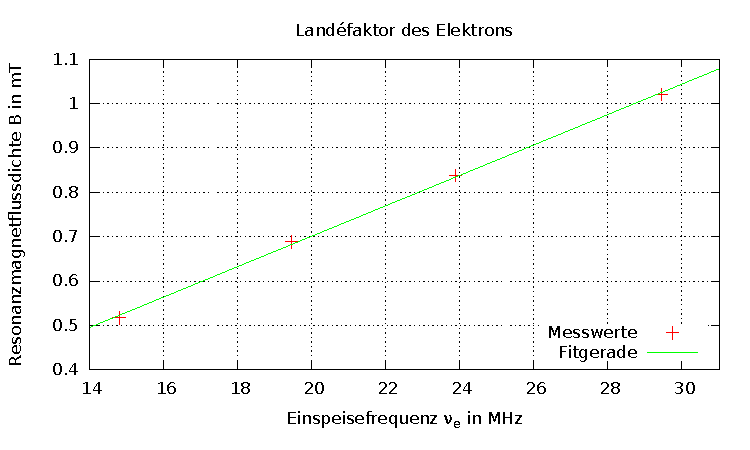
\includegraphics[width=0.8\textwidth]{../pics/landefaktor.pdf}
\caption{Gyromagnetisches Verhältnis oder Landéfaktor des Elektrons}
\label{pic_gyro}
\end{figure}
und zu einem Steigungsparameter 
\begin{equation}
m_\text{gyro} = 0,0343 \pm 0,0006 \text{ Ts}
\end{equation}
führt und damit schließlich den Landéfaktor berechnen lässt.
\begin{equation}
 g = \frac{h}{\mu_B\cdot m_\text{gyro}} = 2,082 \pm 0,037
\end{equation}


\section{Diskussion}
\subsection{Erdmagnetfeld}
Der berechnete Wert für das Erdmagnetfeld steht in folgendem Verhältnis zum Literaturwert \cite{ErdB}
\begin{equation}
 \frac{B_\text{Mess}}{B_\text{Lit}} = 68,3 \%.
\end{equation}
Die etwas hohe Abweichung spricht für eine unpräzise Ausrichtung der Helmholtzspule, was auf die sehr empfindliche Bussole zurückführbar ist, die
auf diverse andere elektrische Geräte reagiert.

\subsection{Landéfaktor}
Das gyromagnetische Verhältnis wurde durch einen Fit ermittelt und hat eine Übereinstimmung zum Literaturwert \cite{Gyro} von
\begin{equation}
 \frac{g_\text{Mess}}{g_\text{Lit}} = 103,4 \%.
\end{equation}
Unabhängig von den Abweichungen vom Erdmagnetfeld ist eine sehr gute Bestimmung des Landéfaktors gelungen. 




\begin{thebibliography}{xxxxxxxxxxxxxxxxx}
 \bibitem[Chemie.de]{ErdB}Form und Stärke des Erdmagnetfelds\\ \href{http://www.chemie.de/lexikon/Erdmagnetfeld.html#Form_und_St.C3.A4rke_des_Erdmagnetfeldes}{chemie.de/lexikon/Erdmagnetfeld}
 \bibitem[Universal Lexikon]{Gyro}Landé-Faktor\\ \href{http://universal\_lexikon.deacademic.com/144745/}{universal\_lexikon.deacademic.com/144745/}
\end{thebibliography}

% ========================================
%	Literaturverzeichnis
% ========================================

%\bibliographystyle{plainnat}			% Bibliographie-Style auswählen
%\bibliography{BIBDATEI}			% Literaturverzeichnis

% ========================================
%	Das Dokument endent
% ========================================

\end{document}
